% Name: Cascade control
% Description: Two nested loops: an outer controller sets the reference for a faster inner loop around the actuator.
% Tags: cascade control, nested loops, control systems

\usetikzlibrary{arrows.meta}

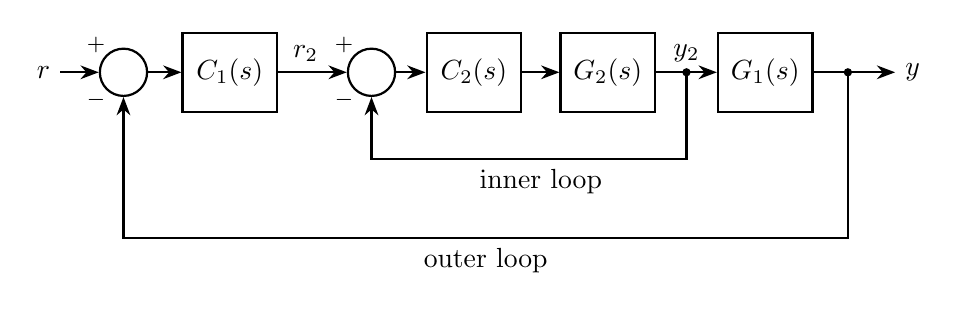
\begin{tikzpicture}[
  block/.style={draw, thick, minimum height=10mm, minimum width=12mm},
  sum/.style={draw, thick, circle, inner sep=0pt, minimum size=6mm},
  arrow/.style={-{Stealth}, thick},
  sign/.style={font=\footnotesize},
  every label/.style={font=\footnotesize, gray!70!black},
]
  \node[sum] (s1) at (0.8,0) {};
  \node[block] (C1) at (2.15,0) {$C_1(s)$};
  \node[sum] (s2) at (3.95,0) {};
  \node[block] (C2) at (5.25,0) {$C_2(s)$};
  \node[block] (G2) at (6.95,0) {$G_2(s)$};
  \node[block] (G1) at (8.95,0) {$G_1(s)$};

  \draw[arrow] (0,0) node[left] {$r$} -- (s1);
  \draw[arrow] (s1) -- (C1);
  \draw[arrow] (C1) -- node[above, pos=0.4] {$r_2$} (s2);
  \draw[arrow] (s2) -- (C2);
  \draw[arrow] (C2) -- (G2);
  \draw[arrow] (G2) -- (G1);
  \draw[arrow] (G1) -- (10.6,0) node[right] {$y$};
  % Inner loop feeds back y2, outer loop feeds back y
  \draw[arrow] (7.95,0) node[above] {$y_2$} |- (6.1,-1.1) node[below, pos=1] {inner loop} -| (s2);
  \draw[arrow] (10,0) |- (5.4,-2.1) node[below, pos=1] {outer loop} -| (s1);
  \fill (7.95,0) circle (1.5pt) (10,0) circle (1.5pt);

  \foreach \s in {s1, s2} {
    \node[sign] at ([shift={(-3.5mm,3.5mm)}]\s) {$+$};
    \node[sign] at ([shift={(-3.5mm,-3.5mm)}]\s) {$-$};
  }
\end{tikzpicture}
